\documentclass{article}

\usepackage{booktabs}
\usepackage{tabularx}
\usepackage{enumerate}
\usepackage{graphicx}
\usepackage{float}
\usepackage{chngpage}
\usepackage[round]{natbib}

\title{Software Requirements Specification\\\progname}

\author{\authname}

\date{}

%% Comments

\usepackage{color}

\newif\ifcomments\commentstrue %displays comments
%\newif\ifcomments\commentsfalse %so that comments do not display

\ifcomments
\newcommand{\authornote}[3]{\textcolor{#1}{[#3 ---#2]}}
\newcommand{\todo}[1]{\textcolor{red}{[TODO: #1]}}
\else
\newcommand{\authornote}[3]{}
\newcommand{\todo}[1]{}
\fi

\newcommand{\wss}[1]{\authornote{blue}{SS}{#1}} 
\newcommand{\plt}[1]{\authornote{magenta}{TPLT}{#1}} %For explanation of the template
\newcommand{\an}[1]{\authornote{cyan}{Author}{#1}}

%% Common Parts

\newcommand{\progname}{ProgName} % PUT YOUR PROGRAM NAME HERE
\newcommand{\authname}{Team \#, Team Name
\\ Student 1 name
\\ Student 2 name
\\ Student 3 name
\\ Student 4 name} % AUTHOR NAMES                  

\usepackage{hyperref}
    \hypersetup{colorlinks=true, linkcolor=blue, citecolor=blue, filecolor=blue,
                urlcolor=blue, unicode=false}
    \urlstyle{same}
                                


\begin{document}

\begin{table}[hp]
\caption{Revision History} \label{TblRevisionHistory}
\begin{tabularx}{\textwidth}{llX}
\toprule
\textbf{Date} & \textbf{Developer(s)} & \textbf{Change}\\
\midrule
10/05/2022 & Namit Chopra, Brandon Duong  & Finished First\\
 & Andrew Balmakund, Mohammad Harun &  Version\\
 & Mihail Serafimovski & \\
\bottomrule
\end{tabularx}
\end{table}

\newpage

\maketitle

\newpage

\pagenumbering{roman}
\tableofcontents
\listoftables
\listoffigures

\newpage

\pagenumbering{arabic}

This document describes the requirements for Farming Matters. The template for the Software
Requirements Specification (SRS) is a subset of the Volere ~\citep{RobertsonAndRobertson2012} template. \newline \\ Some modifications made to the Volere subset template are:
\begin{itemize}
    \item (Added) Section 3.10: Requirements that are likely/unlikely to change
    \item (Added) Section 4: Traceability matrix
    \item (Added) Section 5.5: Requirements Phase-In Plan
    \item (Added) Section 6.1: Team technologies/skills - Reflection
    \item (Removed) Section 5.11 Ideas for Solutions - Ideas for solutions are represented in the risks section, as mitigation is provided for each risk.
\end{itemize}



\section{Project Drivers}

\subsection{The Purpose of the Project}
The purpose of this project is to conduct survey research through an interactive and engaging activity. This will further help understand genuine decisions from the users to help with the research of understanding risk-making decisions.


\subsection{The Stakeholders}

\subsubsection{The Client}
The client of this project is Dr.Yiannakoulias who is the supervisor of this project. Dr.Yiannakoulias is part of the School of Earth, Environment and Society at McMaster University.

\subsubsection{The Customers}
The customers of the project are individuals that enjoy management and role-playing simulation games. As well as individuals willing to be a respondent to help conduct data for research.

\subsubsection{Other Stakeholders}
Other stakeholders would include the Ethics board. Some of the requirements regarding data collection are derived from this stakeholder. They also have to approve the final product to check if there are any ethical issues.

\subsection{Mandated Constraints}

\begin{itemize}
    \item Description: The project shall have a budget of \$0.\\
    \textbf{Rationale:} The developers of the project have no budget for this project. The professor might purchase game assets if he wishes to change the look of the game after the game has been created.\\ 
    Fit Criterion: The developer team should use open source and free software.
    \item Description: The project shall run properly on different operating systems like Linux, Windows and Mac OS.\\
    \textbf{Rationale:} The project shall be portable.\\
    Fit Criterion: The user shall be able to run the game on different operating systems.
\end{itemize}

\subsection{Naming Conventions and Terminology}
\begin{itemize}
    \item Player: The user playing the game. The player or user is the participant and focus of the study.
    \item Land: An area where the user can interact with the farm. This includes planting crops, fertilizing crops and adding buildings.
    \item Inventory: Where the user will be able to store items.
    \item Items: The user will be able to acquire these into their inventory, including grown crops, crop seeds, and fertilizers.
    \item Focus groups: A set of users will be involved with discrete decision-making and another set of users will be involved with probabilistic decision-making.
    \item Turns: these are rounds that happen per season where a decision can be made. 
    \item Seasons: Including Winter, Spring, Summer, and Fall. The current season changes depending on the turn number, and has an effect on which crops can be grown. Each season lasts SEASON\_LENGTH turns.
    \item Key Questions: These are the compulsory questions that will be asked to the user. The first will be whether the user wants to pay the consultant for advice. The second question will ask the user if they want to purchase insurance for crops.
\end{itemize}
\subsection{Relevant Facts and Assumptions about User Characteristics}

The user should have the physical and visual ability to operate a computer. This includes actions such as clicking a mouse and pressing buttons on the keyboard. The user should be familiar with the hardware they are using, in this case, a desktop or laptop. It would be preferable if the user had some knowledge of the basic idea of farming; however, there will be a tutorial to go over the basic rules of the game if they lack sufficient knowledge on how to play. 
\\ Due to the research-oriented nature of the project and the ethical requirements, all users will be over the age of 18.

\section{Functional Requirements}

\subsection{The Scope of the Work and the Product}

\subsubsection{The Context of the Work}
The Farming Matters game will create interactive and engaging management and role-playing game. The user will be provided with risk-making decisions involving the management of their own farm. The game will involve in-game currency where users will have the ability to buy and sell items from an in-game shop. The system will also track and save each user's decisions which will be available for them to see at the end of each turn. The user will also have the ability to customize their farm layout and place items within their available land. 

\begin{figure}[!htb]
    \centering
    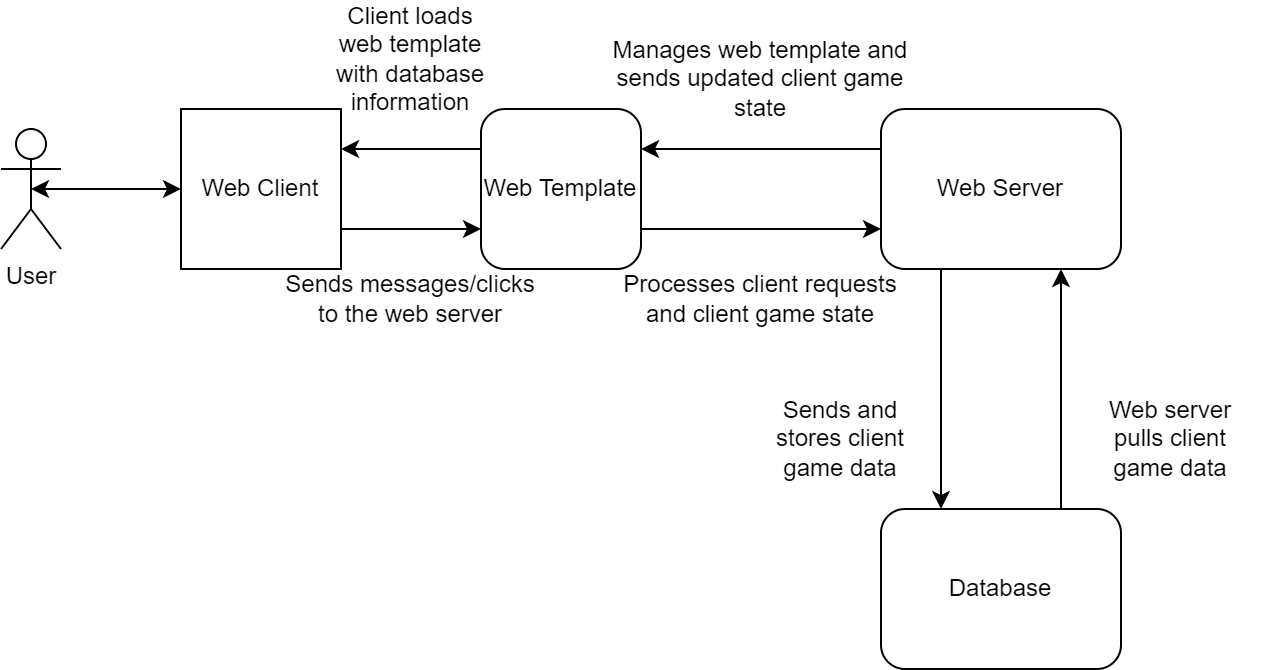
\includegraphics[width=14cm]{context.png}
    \caption{Web Application Context Diagram. This diagram demonstrates the system's external boundary, that being the user interacting with the web client.}
    \label{fig:context_diagram}
\end{figure}
\newpage

\subsubsection{Work Partitioning}
\begin{table}[h]
    \centering
    \begin{tabular}{|p{0.33\linewidth} | p{0.33\linewidth} | p{0.33\linewidth}| }
    \hline
         Event & Input/Output & Summary \\
         \hline
         User ends turn & Input: user selects end turn option & System responds and update current game state\\
         \hline 
         Collect user decisions & Input: all prior user decisions, users progression and focus group \newline Output: Group data based on focus group  & System provides organized data \\
         \hline 
          User creates account & Input: Username and password \newline Output: Associated account & The user inputs their desired username and password and the system creates an account and stores the credentials\\
         \hline 
         User requests to delete their data & Input: Username and password \newline Output: Associated account and all its data is deleted & The user inputs their account's username and password and the system deletes the associated account and all its corresponding data\\
         \hline 
    \end{tabular}
    \caption{Work Partitioning Table}
    \label{tab:my_label}
\end{table}

\subsubsection{Individual Product Use Cases and Undesired Event Handling}

\textbf{Use case \#1:} User creates account\\
\textbf{Primary Actor:} User\\
\textbf{Supporting Actors:} None\\
\textbf{Precondition:} The user has completed the consent form\\
\textbf{Trigger:} The user is directed to the create account page\\
\textbf{Main Success Scenario}
\begin{enumerate}
    \item User is on the home page and selects to create account
    \item User is on the create account page
    \item User provides the required information
    \item System verifies all required information has been provided
    \item User completes human verification task
    \item System validates human verification
    \item System securely registers user information
    \item User is redirected back to the Home page
\end{enumerate}
\textbf{Secondary Scenarios}:
\begin{enumerate}
    \item User fails to provide the required information: one or more fields have not been provided by the user
    \item User fails human verification task: user has failed a human verification test which either means they entered in the wrong details or an automated script attack for account creation occurred

\end{enumerate}
\textbf{Success Postcondition:} The user has successfully created an account and account information is stored and secured in a database.


\noindent\\
\textbf{Use case \#2:} User signs into account\\
\textbf{Primary Actor:} User\\
\textbf{Supporting Actors:} None\\
\textbf{Precondition:} The user has successfully created an account\\
\textbf{Trigger:} The user arrives at the login page\\
\textbf{Main Success Scenario}
\begin{enumerate}
    \item User is on the home page and selects to login
    \item User is on the login page
    \item User provides the required information
    \item System verifies all required information has been provided
    \item User is redirected to the Home page as a logged in user
\end{enumerate}
\textbf{Secondary Scenarios}:
\begin{enumerate}
    \item Login unsuccessful: the provided login details do not match any login details in the database
\end{enumerate}
\textbf{Success Postcondition:} The user has successfully logged into their created account and their game state is loaded from the database. \newline

\noindent\\
\textbf{Use case \#3:} User logs out of their account\\
\textbf{Primary Actor:} User\\
\textbf{Supporting Actors:} None\\
\textbf{Precondition:} The user has successfully created an account and is currently logged in\\
\textbf{Trigger:} The user has selected an option to logout\\
\textbf{Main Success Scenario}
\begin{enumerate}
    \item User accesses and selects the logout option
    \item User is presented with a confirmation page to logout
    \item User selects logout option
    \item System shall save all progress made in the current session and append to their overall progression that is stored in the database
    \item User is redirected to Home page
\end{enumerate}
\textbf{Secondary Scenarios}:
\begin{enumerate}
    \item User is inactive: After INACTIVE\_TIME period, the system shall log out the user automatically. Perhaps they may have closed the tab running the web application and have not returned for a while
\end{enumerate}
\textbf{Success Postcondition:} The user has successfully logged out of the system and all logged data has been stored successfully. \newline


\noindent\\
\textbf{Use case \#4:} User retrieves forgotten password\\
\textbf{Primary Actor:} User\\
\textbf{Supporting Actors:} None\\
\textbf{Precondition:} The user has successfully created an account\\
\textbf{Trigger:} The user has selected an option to forget password\\
\textbf{Main Success Scenario}
\begin{enumerate}
    \item User accesses login page and selection forget password option
    \item User enters required information to gain back access to account
    \item System sends the users follow up details to confirm the legitimacy of their account
    \item User is able to provide a new password
    \item System shall update the password of the current user in the database 
    \item User is redirected to the Home page as a logged in user
\end{enumerate}
\textbf{Secondary Scenarios}:
\begin{enumerate}
    \item System unable to verify account details: User may have entered the incorrect details needed to obtain back access to the account. They may also pretend to be someone else but is not able to gain access to the account
\end{enumerate}
\textbf{Success Postcondition:} The user has successfully updated their account details and is logged in. \newline

\noindent\\
\textbf{Use case \#5:} User opts out to delete their data\\
\textbf{Primary Actor:} User\\
\textbf{Supporting Actors:} None\\
\textbf{Precondition:} The user has successfully created an account and is currently signed in\\
\textbf{Trigger:} The user has selected an option to delete their data\\
\textbf{Main Success Scenario}
\begin{enumerate}
    \item User accesses selection to delete data
    \item System logs the user out
    \item System deleted all data belonging to the user
    \item User is redirected to the Home page
\end{enumerate}
\textbf{Secondary Scenarios}:
None\\
\textbf{Success Postcondition:} The user has successfully opted out to delete their data and is no longer stored in the database. \newline


\noindent\\
\newpage
\textbf{Use case\# 6:} User completes a turn\\
\begin{figure}[H]
    \centering
    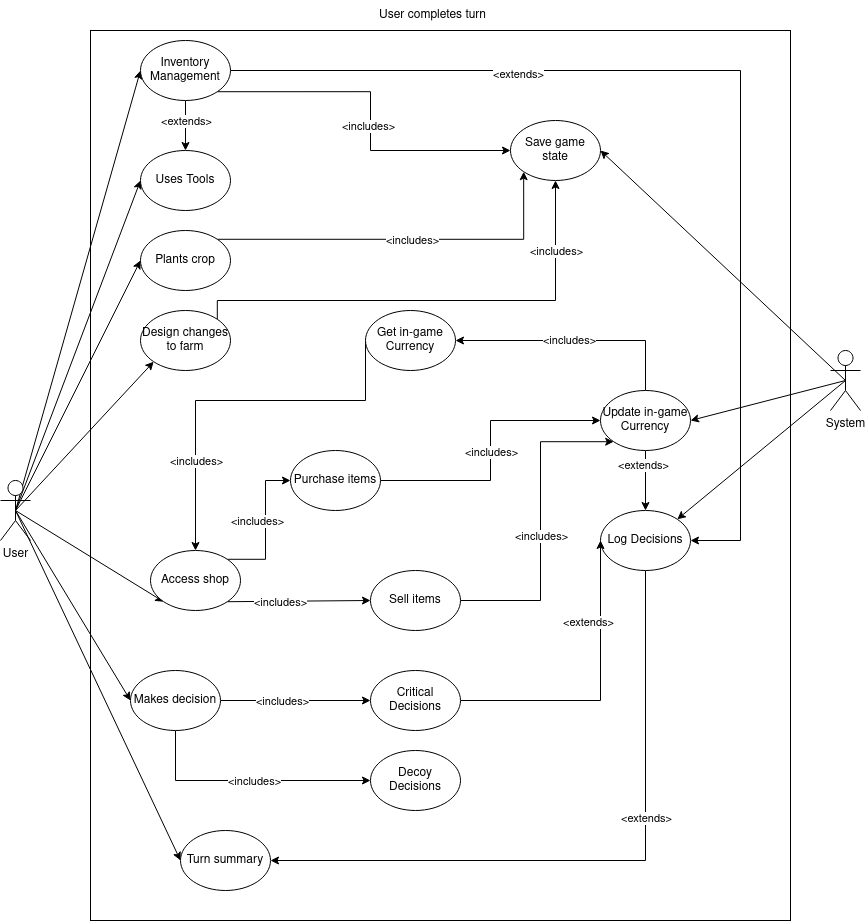
\includegraphics[width=12cm]{srs_usecase.drawio.png}
    \caption{Use Case \#6: User completes a turn}
    \label{fig:context_diagram}
\end{figure}
\newpage
%%% new subsection
\subsection{Functional Requirements}
\begin{enumerate}[{FR}1. ]
    %Other
    \item \label{FR1} The system must allow users to create an account.\\
    \textbf{Rationale}: The purpose of the game is to track user decisions and be able to see which participant did what decision. For this to happen, users must be associated to with an account.
    \item \label{FR2} The system must allow the user to reset their password.\\
    \textbf{Rationale}: It is possible a user misplaces their password and loses all their account progress. This effectively removes the participant from the study and so this must be rectified.
    \item \label{FR3} The system must allow users to accumulate in-game currency.\\
    \textbf{Rationale}: In-game currency acts as a performance metric, and also helps engage the player in planning ahead for their future decisions. Optimizing what one should spend their in-game currency on is both parts of the study and the engagement of the game itself.
    \item \label{FR4} The system must allow the user to store their items in an inventory.
    \textbf{Rationale}: The user must be able to view the items they currently own.
    \item \label{FR5} The system must verify new users as humans.\\
    \textbf{Rationale}: As anyone can make an account, the system is susceptible to related attacks. The system verifying a user as a human before creating their account may slow down these attempts.
    %Shop related
    \item \label{FR6} The system must allow users to purchase items from a shop.\\
    \textbf{Rationale}: Helps engage the player with the feeling of progression and decision-making.
    %\item The system must allow users to buy crop seeds\\
    %\textbf{Rationale}: Helps engage the player with the feeling of progression and decision-making
    \item \label{FR7} The system must allow users to grow crops on owned land.\\
    \textbf{Rationale}: Helps engage the player with the feeling of progression and decision-making.
    \item \label{FR8} The system must allow users to sell crops at a fluctuating price. The fluctuating price will be determined by a base price $p_b$ for the crop, plus or minus a random factor $r$ within one third of the base price. In mathematical terms, the fluctuating price is given by \\ $f(p_b) = p_b + r*(p_b/3)$, where $-1 \le r \le 1$.\\
    \textbf{Rationale}: Helps engage the player with the feeling of progression and decision-making.
    %\item The system must allow users to buy fertilizer\\
    %\textbf{Rationale}: Helps engage the player with the feeling of progression and decision-making
    \item \label{FR9} The system must allow users to use fertilizer on planted crops.\\
    \textbf{Rationale}: Helps engage the player with the feel of progression and decision-making.
    %Playing the game
    \item \label{FR10} The system must allow users to buy land.\\
    \textbf{Rationale}: Helps engage the player with the feel of progression and decision-making.
    \item \label{FR11} The system must prompt users for consulting advice every CONSULTING\_INTERVAL turns.\\
    \textbf{Rationale}: This decision is one of the two key questions the research is looking at. Whether people are willing to pay for information, and for what information (i.e deterministic or probabilistic).
    \item \label{FR12} The system must prompt users for insurance for planted crops.\\
    \textbf{Rationale}: This decision is the second of the two key questions the research is looking at. Whether people are willing to pay for insurance, and in what circumstance (i.e from the start, or only after they've been affected by an insurable event).
    \item \label{FR13} The system must be able to log user decisions.\\
    \textbf{Rationale}: This was a crucial requirement that was provided by Dr.Yiannakoulias who will be able to view these logs to analyze the data.
    \item \label{FR14} The system must be able to save the user game state.\\
    \textbf{Rationale}: This will give users the option to continue where they left off if they want to continue playing at another time.
    \item \label{FR15} The system must allow users to delete their data.\\
    \textbf{Rationale}: This is a requirement from the ethics board and it is mandatory that users be given this option.
    \item \label{FR16} The system must have a defined area of land for users to manage the farm.\\
    \textbf{Rationale}: This will provide an environment in which players can visualize and interact with their farm.
    \item \label{FR17} The system must allow users to place buildings and items on their land.\\
    \textbf{Rationale}: This will give the user more variability and options in terms of how they want to build their farm.
    \item \label{FR18} The system must present the consent form to participate in the study before starting the game.\\
    \textbf{Rationale}: This is another requirement from both the Ethics board and Dr.Yiannakoulias, and made this a point to emphasize.
    \item \label{FR19} The system must be able to evaluate the total worth of a user's assets. In mathematical terms, $W = \displaystyle\sum_{a \in A}^{}a.value$, where $W$ is the total worth of the user's assets, and A represents all of the player's assets. \\ $A = $ currency $ \cup $ inventory $ \cup $ land $ \cup $ buildings.  \\
    \textbf{Rationale}: Total worth of all a user's assets acts as a performance metric, and also helps engage the player by allowing them to see how much they've progressed.
    \item \label{FR20} The system must be able to assign a user to a specific focus group.\\
    \textbf{Rationale}: This is essential for the research study to demonstrate whether or not people prefer deterministic or probabilistic information.
    \item \label{FR21} The system must include random events to occur EVENT\_OCCURRENCE.\\
    \textbf{Rationale}: Helps engage the player by needing them to plan ahead for the possible unknown.
    \item \label{FR22} The system must have the current season change over time.\\
    \textbf{Rationale}: Helps engage the player as they must plan ahead for what is possible during the different seasons in terms of what to plant, and what risks there are within each season.
\end{enumerate}

\subsection{Requirements That Are Likely/Unlikely to Change}
\begin{table}[H]
    \centering
    \begin{tabular}{|p{0.40\linewidth} | p{0.40\linewidth}|}
    \hline
         Likely & Unlikely \\
         \hline
         FR2, FR5, FR19, FR21 & FR1, FR3, FR4, FR6, FR7, FR8, FR9, FR10, FR11, FR12, FR13, FR14, FR15, FR16, FR17, FR18, FR20, FR22    \\
         \hline
    \end{tabular}
    \caption{Likely/Unlikely to Change Table}
    \label{tab:my_label}
\end{table}
\begin{itemize}
    \item FR1: This is unlikely to change as accounts are needed to associate a specific user to their game state
    \item FR3, FR4, FR6, FR7, FR8, FR9, FR10, F14, FR16, F17, FR21, FR22: These are unlikely to change as these are the basic core game mechanics that define the desired game loop
    \item FR11, FR12, FR13, FR20: These are unlikely to change as they implement the essentials behind the research study aspect
    \item FR15, F18: This is unlikely to change because it is required for the ethics board to approve the game. The approval of the game by the ethics board is a must.
    
\end{itemize}

\section{Non-functional Requirements}

\subsection{Look and Feel Requirements}
\begin{enumerate}[{LF}1. ]
    \item The menu shall be minimalistic. \\
    \textbf{Fit Criteria}: The menu should only require the necessary elements and not overwhelm the user.
    \item The menu and game interface shall follow a consistent theme. \\
    \textbf{Fit Criteria}: All visual assets should include the same colors and style across all aspects of the game.  
    \item The system must have engaging audio. \\
    \textbf{Fit Criteria}: Survey a group of individuals and 90\% of them should be satisfied with the audio assets. 
    \item The system must have engaging graphics.\\
    \textbf{Fit Criteria}: Survey a group of individuals and 90\% of them should be satisfied with the graphical assets.
    \item The system must be responsive on monitors at least MIN\_MONITOR. \\
    \textbf{Fit Criteria}: All aspects of the system should be functioning accordingly and be responding at the resolution set to MIN\_MONITOR.
    \item The system must have engaging gameplay. \\
    \textbf{Fit Criteria}: Average number of turns played is MIN\_TURNS.
    
\end{enumerate}

\subsection{Usability and Humanity Requirements}
\begin{enumerate}[{UH}1. ]
    \item The system must be easy to learn for people aged AGE\_GROUP. \\
    \textbf{Fit Criteria}: Survey a group of individuals and 95\% of them should easily understand the in-game logic, understand the information provided to them and be able to interact with all the menus.
\end{enumerate}

\subsection{Performance Requirements}
\begin{enumerate}[{PR}1. ]
    \item The website must load within LOAD\_TIME seconds. \\
    \textbf{Fit Criteria}: The measured time from the user sending an initial request to access the website and the website loading is less than or equal to LOAD\_TIME.
    
    \item The website must respond to any user interaction within RESPONSE\_TIME seconds. \\
    \textbf{Fit Criteria}: The measured time from the user interacting with the website and the website providing the user with some response is less than or equal to RESPONSE\_TIME.
\end{enumerate}

\subsection{Operational and Environmental Requirements}
\begin{enumerate}[{OE}1. ]
    \item The system must be functional on modern browsers. \\
    \textbf{Fit Criteria}: The user shall be able to run the game on different modern browsers such as Google Chrome, Firefox, Microsoft Edge.
    
    \item The system must be functional on any version of the browser it's used on released within the past SUPPORTED\_VERSIONS. \\
    \textbf{Fit Criteria}: The user shall be able to run the game on any supported version of their browser of choice (so long as their browser is supported).
\end{enumerate}


\subsection{Maintainability and Support Requirements}
\begin{enumerate}[{MR}1. ]
    \label{MR1}
    \item The system must allow assets to be replaced. \\
    \textbf{Fit Criteria}: The development team and client shall be able to change any visual or audio assets with ease and not disrupt any part of the system.
\end{enumerate}

\subsection{Security Requirements}
\begin{enumerate}[{SR}1. ]
    \item The system must not allow automation of creating accounts. \\
    \textbf{Fit Criteria}: There should be measures in place to prevent automated attacks. \\
    
\end{enumerate}
\subsection{Cultural Requirements}
N.A.
\subsection{Legal Requirements}
\begin{enumerate}[{LR}1. ]
    \item The system must not keep data if a user retracts consent. \\
    \textbf{Fit Criteria}:  Upon request to delete data, there should be no instance of the user's data in the database.
\end{enumerate}

\subsection{Health and Safety Requirements}
N.A.\\

\subsection{Requirements That Are Likely/Unlikely to Change}
\begin{table}[h]
    \centering
    \begin{tabular}{|p{0.40\linewidth} | p{0.40\linewidth}|}
    \hline
         Likely & Unlikely \\
         \hline
         PR1, PR2, SR1 & LF1, LF2, LF3, LF4, LF5, LF6, UH1, OE1, OE2, MR1, LR1      \\
         \hline
    \end{tabular}
    \caption{Likely/Unlikely to Change Table}
    \label{tab:my_label}
\end{table}
\begin{itemize}
    \item LF1, LF2, LF3, LF4, LF6: These are unlikely to change as these are needed to fully immerse the user within the game and not think about the underlying research (to ensure genuine results).
    \item LF5, UH1, OE1, OE2: This is unlikely to change as these tackle the problem of having the application as accessible as possible.
    \item MR1: This is unlikely to change as it allows Dr.Yiannakoulias to tweak and further improve upon the finished product.
    \item LR1: This is unlikely to change as this is required for the ethics board to approve the finished product.
    
\end{itemize}
\section{Traceability Matrix}

The traceability matrix below shows the relationships between functional requirements and non-functional requirements/risks. Any cells with a 'Y' trace to each other. 

\begin{table}[H]
\begin{adjustwidth}{-1.87in}{-1in}
\begin{tabular}{c|c|c|c|c|c|c|c|c|c|c|c|c|c|c|c|c|c|c|}
\cline{2-19}
                                    & \textbf{LF1} & \textbf{LF2} & \textbf{LF3} & \textbf{LF4} & \textbf{LF5} & \textbf{LF6} & \textbf{UH1} & \textbf{PR1} & \textbf{PR2} & \textbf{OE1} & \textbf{OE2} & \textbf{MS1} & \textbf{SR1} & \textbf{LR1} & \textbf{R1} & \textbf{R2} & \textbf{R3} & \textbf{R4} \\ \hline
\multicolumn{1}{|c|}{\textbf{FR1}}  &              &              &              &              &              &              &              &              &              &              &              &              & Y            &              &             &             &             &             \\ \hline
\multicolumn{1}{|c|}{\textbf{FR2}}  &              &              &              &              &              &              &              &              &              &              &              &              &              &              &             &             &             &             \\ \hline
\multicolumn{1}{|c|}{\textbf{FR3}}  &              &              &              &              &              & Y            &              &              &              &              &              &              &              &              &             &             &             &             \\ \hline
\multicolumn{1}{|c|}{\textbf{FR4}}  &              &              &              &              &              &              &              &              &              &              &              &              &              &              &             &             &             &             \\ \hline
\multicolumn{1}{|c|}{\textbf{FR5}}  &              &              &              &              &              &              &              &              &              &              &              &              &              &              &             &             &             &             \\ \hline
\multicolumn{1}{|c|}{\textbf{FR6}}  &              &              &              &              &              & Y            &              &              &              &              &              &              &              &              &             &             &             &             \\ \hline
\multicolumn{1}{|c|}{\textbf{FR7}}  &              &              &              &              &              & Y            &              &              &              &              &              &              &              &              &             &             &             &             \\ \hline
\multicolumn{1}{|c|}{\textbf{FR8}}  &              &              &              &              &              & Y            &              &              &              &              &              &              &              &              &             &             &             &             \\ \hline
\multicolumn{1}{|c|}{\textbf{FR9}}  &              &              &              &              &              & Y            &              &              &              &              &              &              &              &              &             &             &             &             \\ \hline
\multicolumn{1}{|c|}{\textbf{FR10}} &              &              &              &              &              & Y            &              &              &              &              &              &              &              &              &             &             &             &             \\ \hline
\multicolumn{1}{|c|}{\textbf{FR11}} &              &              &              &              &              &              &              &              &              &              &              &              &              &              &             &             &             &             \\ \hline
\multicolumn{1}{|c|}{\textbf{FR12}} &              &              &              &              &              &              &              &              &              &              &              &              &              &              &             &             &             &             \\ \hline
\multicolumn{1}{|c|}{\textbf{FR13}} &              &              &              &              &              &              &              &              &              &              &              &              &              &              &             &             &             &             \\ \hline
\multicolumn{1}{|c|}{\textbf{FR14}} &              &              &              &              &              &              &              &              &              &              &              &              &              &              &             &             &             &             \\ \hline
\multicolumn{1}{|c|}{\textbf{FR15}} &              &              &              &              &              &              &              &              &              &              &              &              &              & Y            &             & Y           &             &             \\ \hline
\multicolumn{1}{|c|}{\textbf{FR16}} &              &              &              &              &              & Y            &              &              &              &              &              &              &              &              &             &             &             &             \\ \hline
\multicolumn{1}{|c|}{\textbf{FR17}} &              &              &              &              &              & Y            &              &              &              &              &              &              &              &              &             &             &             &             \\ \hline
\multicolumn{1}{|c|}{\textbf{FR18}} &              &              &              &              &              &              &              &              &              &              &              &              &              &              &             & Y           &             &             \\ \hline
\multicolumn{1}{|c|}{\textbf{FR19}} &              &              &              &              &              &              &              &              &              &              &              &              &              &              &             &             &             &             \\ \hline
\multicolumn{1}{|c|}{\textbf{FR20}} &              &              &              &              &              &              &              &              &              &              &              &              &              &              &             &             &             &             \\ \hline
\multicolumn{1}{|c|}{\textbf{FR21}} &              &              &              &              &              & Y            &              &              &              &              &              &              &              &              &             &             &             &             \\ \hline
\multicolumn{1}{|c|}{\textbf{FR22}} &              &              &              &              &              &              &              &              &              &              &              &              &              &              &             &             &             &             \\ \hline
\multicolumn{1}{|c|}{\textbf{R1}}   &              &              &              &              &              &              &              &              &              &              &              &              &              &              &             &             &             &             \\ \hline
\multicolumn{1}{|c|}{\textbf{R2}}   &              &              &              &              &              &              &              &              &              &              &              &              &              &              &             &             &             &             \\ \hline
\multicolumn{1}{|c|}{\textbf{R3}}   &              &              & Y            & Y            &              & Y            &              &              &              &              &              &              &              &              &             &             &             &             \\ \hline
\multicolumn{1}{|c|}{\textbf{R4}}   &              &              &              &              &              &              &              &              &              &              &              &              &              &              &             &             &             &             \\ \hline
\end{tabular}
\caption{Traceability Matrix}
    \label{tab:my_label}
\end{adjustwidth}
\end{table}



\section{Project Issues}

\subsection{Open Issues}
N/A

\subsection{Off-the-Shelf Solutions}
Although there are games that are themed around farming, they do not provide all the aspects required for this project. Games like FarmVille provide an entertaining and engaging way to manage a farm. However, they do not provide information about user decisions nor are they targeted toward research. 

There are also lab experiments and surveys used for collecting data for the specified research area. The results from these methods often do not accurate information about how humans make decisions in real life. The subjects tend to complete these methods for the incentive which results in an inaccurate collection of data.

There aren't any off-the-shelf solutions available that address all aspects of this problem. The game must be engaging and collect information about risk vs reward decisions in managing a farm. The information collected must also match the format which can be used for research. The combination of information collection, an engaging game, and visibility of logged information is unavailable off-the-shelf.

\subsection{New Problems}
\subsubsection{Effects on the Current Environment}
The game will be graphics intensive which may contribute to a lag on certain devices. This will be exacerbated if the machine is running numerous other applications. The main game decisions also need to be logged into a database which may contribute to a lag as well.

\subsubsection{Effects on the Installed Systems}
N/A

\subsubsection{Potential User Problems}
The learning curve play is an important factor that determines how many users play the game. As the game should depict real-life decisions needed to manage a farm, the game may be complex and contain many different aspects. Failure to provide an informative guide may result in a lack of understanding of how to play the game. Furthermore, it may also result in many users quitting before they have made any progress in the game.


\subsubsection{Limitations in the Anticipated Implementation Environment That May Inhibit the New Product}
A browser and an internet connection are required to play the game. It is not uncommon for one to lose an internet connection while using the browser. Users may experience a loss of connection as they are playing the game which will limit the product. The user may be able to interact with the interface of the game; however, none of the decisions will be logged nor will the game state be saved.

\subsubsection{Follow-Up Problems}
There will be a risk if the libraries get updated during the development. This may result in in-game features being unable to run or load.

The research may need to be updated that better targets the information being searched for in the game. The game may not be providing the information that is useful to the research. The game may need to be re-designed to better obtain the information needed for the research area.


\subsection{Tasks}
The following is the link to our project schedule and all task deadlines:
\href{https://github.com/brandonduong/Farming-Matters/blob/main/docs/Schedule/FarmingMattersSchedule.pdf}{\textit{Gantt chart}}.

\subsection{Requirements Phase-In Plan}
\begin{table}[H]
\centering
\begin{tabular}{|l|l|l|ll}
\cline{1-3}
\textbf{Requirements} & \textbf{Priority} & \textbf{Deadline} &  &  \\ \cline{1-3}
\hyperref[FR1]{FR1}          & High     & Dec. 1, 2022      &  &  \\ \cline{1-3}
\hyperref[FR2]{FR2}          & Low      & Jan. 31, 2023     &  &  \\ \cline{1-3}
\hyperref[FR3]{FR3}          & High     & Dec. 1, 2022      &  &  \\ \cline{1-3}
\hyperref[FR4]{FR4}          & Medium   & Jan. 9, 2023      &  &  \\ \cline{1-3}
\hyperref[FR5]{FR5}          & Low      & Jan. 9, 2023      &  &  \\ \cline{1-3}
\hyperref[FR6]{FR6}          & High     & Dec. 31, 2022     &  &  \\ \cline{1-3}
\hyperref[FR7]{FR7}          & High     & Nov. 14, 2022     &  &  \\ \cline{1-3}
\hyperref[FR8]{FR8}          & Medium   & Jan. 9, 2023      &  &  \\ \cline{1-3}
\hyperref[FR9]{FR9}          & Low      & Jan, 31, 2023     &  &  \\ \cline{1-3}
\hyperref[FR10]{FR10}         & Low      & Jan. 9, 2023      &  &  \\ \cline{1-3}
\hyperref[FR11]{FR11}         & High     & Nov. 14, 2022     &  &  \\ \cline{1-3}
\hyperref[FR12]{FR12}         & High     & Nov. 14, 2022     &  &  \\ \cline{1-3}
\hyperref[FR13]{FR13}         & High     & Nov. 14, 2022     &  &  \\ \cline{1-3}
\hyperref[FR14]{FR14}         & High     & Dec. 31, 2022     &  &  \\ \cline{1-3}
\hyperref[FR15]{FR15}         & High     & Jan. 9, 2023      &  &  \\ \cline{1-3}
\hyperref[FR16]{FR16}         & High     & Nov. 14, 2022     &  &  \\ \cline{1-3}
\hyperref[FR17]{FR17}         & Low      & Jan. 9, 2023      &  &  \\ \cline{1-3}
\hyperref[FR18]{FR18}         & High     & Jan. 9, 2023      &  &  \\ \cline{1-3}
\hyperref[FR19]{FR19}         & High     & Dec. 31, 2022     &  &  \\ \cline{1-3}
\hyperref[FR20]{FR20}         & High     & Nov. 14, 2022     &  &  \\ \cline{1-3}
\hyperref[FR21]{FR21}         & Medium   & Jan. 9, 2023      &  &  \\ \cline{1-3}
\hyperref[FR22]{FR22}         & Medium   & Jan. 9, 2023      &  &  \\ \cline{1-3}
\end{tabular}
\end{table}

\subsection{Migration to the New Product}
N/A

\subsection{Risks}
\begin{enumerate}[{R}1.]
    \item Research data is biased by non-research player decisions 
    \\ \textbf{Description:} There are certain decisions in the game which are fundamental for research and must be unbiased. There is a risk that non-fundamental decisions in the game could introduce bias in the way the players respond to the research decisions. This has a medium probability of occurring.
    \\ \textbf{Mitigation:} The research decisions will be indistinguishable from the non-research decisions. This will result in unbiased responses. 
    
    \item Ethics board does not approve the project
    \\ \textbf{Description:} In order for the game to be used as a research tool, it must be approved by a regulatory ethics board. There is an extremely minor risk that the ethics board could not approve the project after the game is made.
    \\ \textbf{Mitigation:} Our supervisor is very knowledgeable about the ethics board requirements, so we worked closely with him to capture requirements that would ensure approval. These are requirements \hyperref[FR15]{FR15} and \hyperref[FR18]{FR18}.
    
    \item Game is not immersive
    \\ \textbf{Description:} The entire purpose of the game is to gather research data in a way where the user does not feel as if they are in a research environment. In order to do this, we need to ensure that the user has fun while playing and feels immersed in the game. There is a risk they may not, which would defeat the purpose of the game.
    \\ \textbf{Mitigation:} We are mitigating this risk by adding many gameplay mechanics and features that will ensure the user feels immersed. We are additionally looking at existing popular farming games to see what makes people feel immersed, and incorporating that into our design.
    
    \item Complexity of new technologies
    \\ \textbf{Description:} There is a good amount of technologies that are new to some team members, and new packages and libraries will need to be learned as we start developing. This could result in too much complexity in the project and affect development time.
    \\ \textbf{Mitigation:} Each technology has a designated member of the team who is an expert on it, and that person will assist the rest of the team with the given technology. We will also use all available resources to learn when needed.
\end{enumerate}

\subsection{Costs}
There are two costs for this project. The first is the graphical assets used in the game. We will have to pay an artist to create digital assets in the form of images, icons, etc. for us to use in the game. Based on discussions with the supervisor, the graphics for the game will be 2d. Taking this into account, we did research on the costs of 2d digital art and there are a number of different price models. If we want custom assets, we will either purchase a set of assets, or we will pay an artist hourly to create them. Overall, graphical assets will cost no more than \$300 for a polished game. 
\\ \\
With this being said, we have decided to run the project with zero budget initially, and for that reason, we will use all free graphical assets. If the supervisor decides to pay for assets in the future, the system shall be designed in a way where the assets will be easily replaceable (as captured in \hyperref[MR1]{MR1}).
\\ \\
The second primary cost will be the operating cost of the servers needed to run the backend code. Our supervisor (Dr. Yiannakoulias) said that he would handle the hosting of the code on his end, so we should consider that an external cost (ie. it's not added to the project budget). Regardless, since this project does not need to be scaled to high levels of traffic, the operating costs should be low (less than \$50/year)
\\ \\
All other functionality can be achieved at no cost, by using open source solutions. Therefore, the total cost to the group will be \$0.

\subsection{User Documentation and Training}
Users will be presented with the following documentation and training throughout the game:
\begin{itemize}
    \item \textbf{Menu With Gameplay Help:} The user will be able to access a menu that contains instructions on the overall gameplay, including the goals of the game, the actions that can be done in a turn, how to make money, etc.
    
    \item \textbf{Menu with controls:} The user will be able to access a menu that contains instructions on the controls of the game.
    
    \item \textbf{Tooltips:} Throughout the user's gameplay, any components which do not have a clear purpose will have tooltips when the user hovers over them.
    
    \item \textbf{Ethics Documentation:} The user will be given documentation about the ethics of the research and their consent, as required by the ethics board.
\end{itemize}

\subsection{Waiting Room}
This section serves as a place to keep track of potential future requirements or functionalities that we may not have time to implement.
\begin{itemize}
    
    \item \textbf{Asynchronous multiplayer}: This will be an exciting feature as players will be able to compete with other players in terms of how efficient they were with their turns, and what decisions the other players made. Multiplayer gameplay is usually a feature found in most games today; however, it will be asynchronous so players don't have to wait on others before they can perform actions.
    
    \item \textbf{Mini-games}: This will be a fun in-game feature which aims to keep players enticed. Mini-games could be played for various reasons. This could be an enjoyable option to earn money for buying items required for their farm. It is also an additional feature to keep the users engaged and motivated to continue playing the game. Combined with asynchronous multiplayer, leaderboards could also be introduced to track minigame performance.
    
    \item \textbf{Visualizing Data}: The data logged and sent to databases could be graphed and visualized in many other ways. This would also be useful for analyzing the results of the experiment.
 
\end{itemize}

\bibliographystyle{plainnat}

\newpage

\bibliography{SRS}

\newpage

\section{Appendix}

\subsection{Team technologies/skills - Reflection  }
\begin{enumerate}
    \item \textbf{ReactJS}: To master this technology, the following members will go through an in-depth tutorial on ReactJS \href{https://reactjs.org/tutorial/tutorial.html}{Tutorial: Intro to React} and complete a basic project that can be found on YouTube (i.e Create a basic sign-up/login-page) to exercise different components taught in the ReactJS tutorial.
        \begin{itemize}
            \item Student: Mihail
        \end{itemize}
    
    \item \textbf{Team Management}: To master this skill, the following members will go through an online LinkedIn course about team management and effective team leadership \href{https://www.linkedin.com/learning/topics/leadership-and-management}{Leadership and Management Online Training Courses}. Another approach is to take on a leadership role when completing the mini projects above that will be done in small groups of 3 or 4 for each group. This skill was chosen because team management is a large factor in a project's success that is often overlooked.
        \begin{itemize}
                \item Student: Brandon
            \end{itemize}
    \item \textbf{Web Development}: To master this technology, the following members will go through a series of basic web development fundamentals and concepts such as \href{https://www.w3schools.com/html/default.asp}{HTML Tutorial}, \href{https://www.w3schools.com/css/default.asp}{CSS Tutorial} and \href{https://www.w3schools.com/js/default.asp}{JavaScript Tutorial} provided by W3Schools. As well, a mini project suggested above will be used to demonstrate the understanding and skills learned through the tutorials. This skill was chosen because this member had very little experience with this tech stack and learning this could be helpful for further projects and work.
        \begin{itemize}
                \item Student: Mohammad 
            \end{itemize}
    \item \textbf{ExpressJS}: To master this technology, the following members will go through an in-depth tutorial and documentation \href{https://expressjs.com/}{Express - Node.js Web Application Framework}. As well, a mini project suggested above will be used to demonstrate the understanding and skills learned through the in-depth tutorial and documentation. This technology was chosen because the following members had a small experience with Express.js and would like to further get a better understanding of middleware in web development, routing, and ultimately better at server-side development.
        \begin{itemize}
                \item Student: Andrew 
            \end{itemize}
    \item \textbf{SQL Database}: To master this technology, the following members will go through an in-depth tutorial for \href{https://www.w3schools.com/sql/default.asp}{SQL}. They will also get hands-on experience by working on a mini-project that will leverage SQL to demonstrate the understanding and skills learned through the tutorial. If needed, other team members with prior SQL experience can assist. This technology was chosen as it is relevant to the industry and will be used in the project.
        \begin{itemize}
                \item Student: Namit
            \end{itemize}
\end{enumerate}


\subsection{Symbolic Parameters}

The definition of the requirements will likely call for SYMBOLIC\_CONSTANTS.
Their values are defined in this section for easy maintenance.


\begin{table}[h]
\caption{\bf Symbolic Parameter Table}
\begin{tabular}{|l|p{0.5\linewidth}|l|}
\hline
\multicolumn{1}{|l}{\bfseries Symbolic Parameter} & \multicolumn{1}{|l|}{\bfseries Description} & \multicolumn{1}{l|}{\bfseries Value}\\
\hline
AGE\_GROUP & The age of the users playing the game & 18 and above \\
\hline
MIN\_MONITOR & The minimum supported monitor resolution for responsiveness & 1280 by 720 \\
\hline
INACTIVE\_TIME & The time used to establish an inactive user. No data has been logged or any control inputs (mouse or keyboard) by the user & 15 minutes \\
\hline
LOAD\_TIME & The maximum time allowed for the application to successfully load & 5 seconds \\
\hline
RESPONSE\_TIME & The maximum time allowed for the application to respond to user input & 5 seconds \\
\hline
CONSULTING\_INTERVAL & The number of turns between each consultant visit & 3 turns \\
\hline
EVENT\_OCCURRENCE & The amount of times an event will occur throughout a season & 2/season \\
\hline
SEASON\_LENGTH & The number of turns per season & 3 turns \\
\hline
SUPPORTED\_VERSIONS & The oldest supported version of browsers & 1 year \\
\hline
MIN\_TURNS & The minimum amount of turns played needed for a study participant to be a significant data point & 12 turns \\
\hline
\end{tabular}
\end{table}



\end{document}